
\documentclass[a4paper,12pt]{article}
\usepackage[utf8]{inputenc}
\usepackage[spanish]{babel}
\usepackage{amsmath, amssymb}
\usepackage{graphicx}
\usepackage{geometry}
\usepackage{hyperref}
\usepackage{float}
\usepackage{fancyhdr}
\usepackage{tocloft}
\geometry{margin=2.5cm}

% Encabezado y pie de página
\pagestyle{fancy}
\fancyhf{}
\lhead{Inferencia y Estimación}
\rhead{Universidad de San Andrés}
\cfoot{\thepage}

% Numeración de ecuaciones y figuras por sección
\numberwithin{equation}{section}
\numberwithin{figure}{section}


% Portada formal
\begin{document}
\noindent
\begin{minipage}{\textwidth}
    \centering
    {\scshape\LARGE Universidad de San Andrés \par}
    \vspace{1.2cm}
    {\scshape\Large Inferencia y Estimación\par}
    \vspace{1.2cm}
    {\huge\bfseries Compresión y Descompresión de Imágenes usando PCA\par}
    \vspace{1.5cm}
    {\large
    Catalina Hirsch - 36557 \\ Clara Zavaroni Benoit - 36772 \\ Maylen Antonella Villagran Cardozo - 36758 \\}
    \vspace{1cm}
    {\large \today\par}
\end{minipage}



\begin{abstract}
La realización de este trabajo práctico tiene como objetivo aplicar el método de \textbf{Análisis de Componentes Principales (PCA)} en la compresión de imágenes. Se busca reducir el espacio de almacenamiento minimizando la pérdida de información, conservando los datos que contienen la mayor parte de la varianza. Posteriormente, se descomprime la imagen y se compara con la original para evaluar la calidad de la compresión, utilizando métricas objetivas. El desempeño se evalúa en función de la cantidad de componentes principales utilizados. Finalmente, se discuten los resultados y conclusiones obtenidas.
\end{abstract}


\section{Introducción}
En este informe se estudia la compresión y descompresión de imágenes mediante el método de Análisis de Componentes Principales (PCA). Se analizan las propiedades estadísticas de las imágenes, se implementa el proceso de compresión y reconstrucción, y se evalúa el desempeño en función de la calidad de la imagen reconstruida y el ahorro de espacio.

\section{Ejercicio 1: Correlación}
El propósito de este ejercicio es analizar el comportamiento de los píxeles vecinos en las imágenes utilizadas. En primer lugar, se cargan las imágenes y se convierten a escala de grises. Luego, se divide cada imagen en bloques de 2x1 píxeles contiguos verticalmente. A continuación, se calcula la correlación entre los píxeles de cada bloque y se almacena en un vector. Finalmente, se realiza un gráfico de dispersión de las correlaciones obtenidas para cada imagen. Los resultados se presentan a continuación:

\begin{figure}[H]
    \centering
    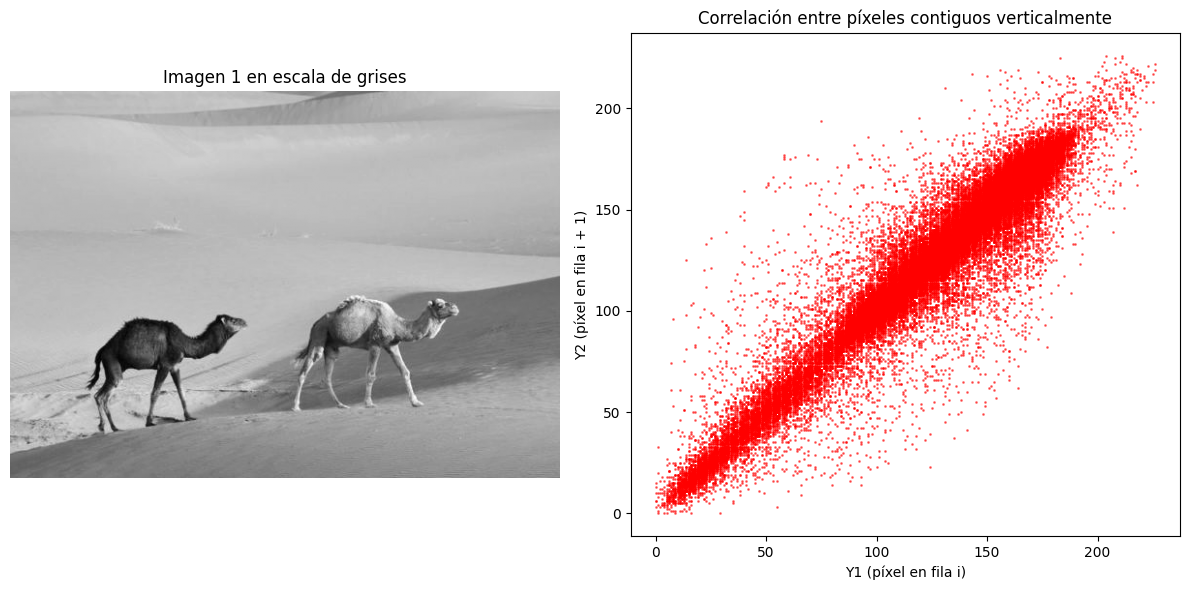
\includegraphics[width=1\textwidth]{Ejercicio1a.png}
    \caption{Imagen 1, gráfico de dispersión de la correlación de píxeles contiguos verticalmente}
    \label{fig:correlacion1}
\end{figure}

Analizando el comportamiento del gráfico, los puntos se alinean en torno a una recta creciente, lo cuál indica una fuerte correlación positiva entre los píxeles.
El resultado se debe a que, la imagen presenta suavidad, el color de los píxeles vecinos se asemeja.

Por otro lado, los resultados de la segunda imagen son los siguientes:

\begin{figure}[H]
    \centering
    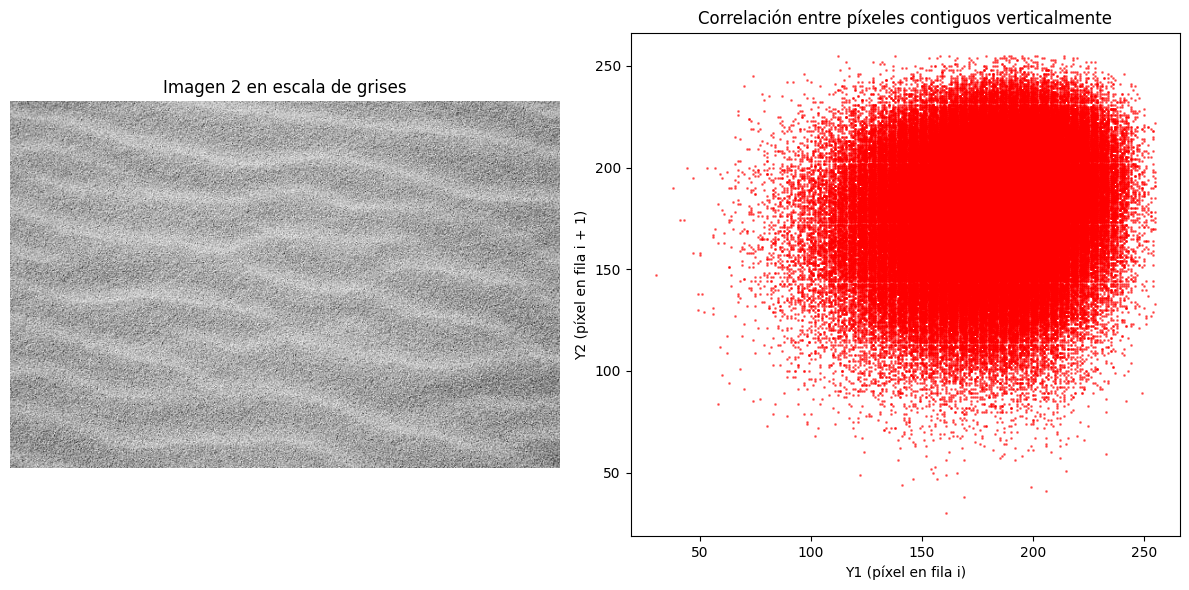
\includegraphics[width=1\textwidth]{Ejercicio1b.png}
    \caption{Imagen 2, gráfico de dispersión de la correlación de píxeles contiguos verticalmente}
    \label{fig:correlacion2}
\end{figure}

A diferencia del gráfico anterior, los puntos se encuentran más dispersos, implicando una correlación más baja que la imagen anterior.
Atribuímos la diferencia al ruido perteneciente a esta imagen, y a la falta de suavidad. Los colores entre los píxeles vecinos no están relacionados.
\\
Luego, se estiman los coeficientes de correlación de cada vector siguiendo el proceso:

\begin{enumerate}
    \item Se separa la imagen en bloques de 8 * 8
    \item Para cada bloque, se utiliza .flatten() para convertir en un vector 64 * 1
    \item Para el calculo de la correlación, se calcula el desvio estándar de cada par de vectores contiguos verticalmente. 
    Evitando la posible división por cero en el calculo.
    \item Se calcula la correlación entre vectores contiguos verticalmente.
\end{enumerate}

Los resultados son los presentados a continuación:
\begin{enumerate}
    \item Para la Imagen 1 se obtuvieron valores como: 
    $[-0.67, -0.69, -0.48, 0.19, \dots]$, 
    con una media de $\bar{\rho}_1 = 0.0993$. 

    \item Para la Imagen 2 los coeficientes fueron: 
    $[0.007, 0.276, -0.017, -0.052, \dots]$, 
    con una media de $\bar{\rho}_2 = 0.0022$.
\end{enumerate}

Los resultados de la primer imagen apoyan lo intuido anteriormente, al aproximarse al valor 1, indican una fuerte correlación entre los píxeles.
Con respecto a la segunda imagen, sus resultados también apoyan lo intuido, al acercase al valor 0, demuestra que los píxeles vecinos no están relacionados.

Por último, se pide una transformación que descorrelacione las variables.
Se utiliza la transformación de descorrelación de PCA:

\[
Y = P^T X
\]
De esta forma, \(Y\) es la proyección de \(X\) en el espacio de autovectores de \(C_X\).
\\
Nuevamente, se hace uso de un gráfico de dispersión por imagen, dando los siguientes resultados:

\begin{figure}[H]
    \centering
    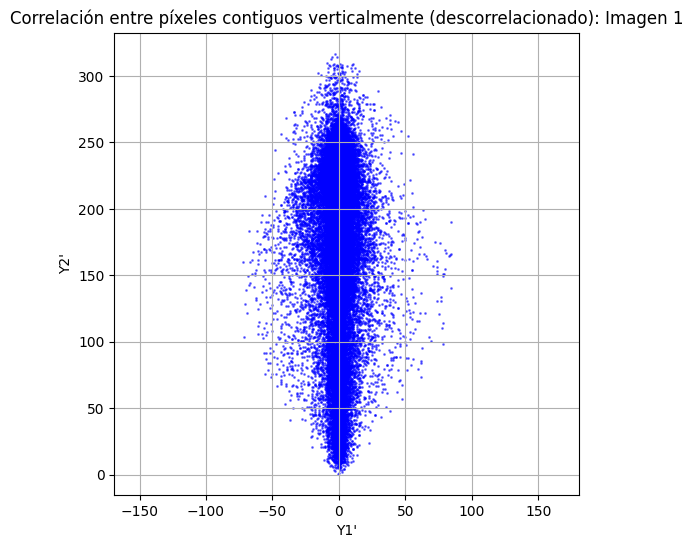
\includegraphics[width=0.7\textwidth]{Ejercicio1c.png}
    \caption{Imagen 1, gráfico de dispersión de la descorrelación de píxeles contiguos verticalmente}
    \label{fig:descorrelacion1}
\end{figure}

Podemos observar en la primer imagen, como los píxeles se encuentran concentrados en el eje vertical Y2, el proceso de descorrelación resulta exitoso.

\begin{figure}[H]
    \centering
    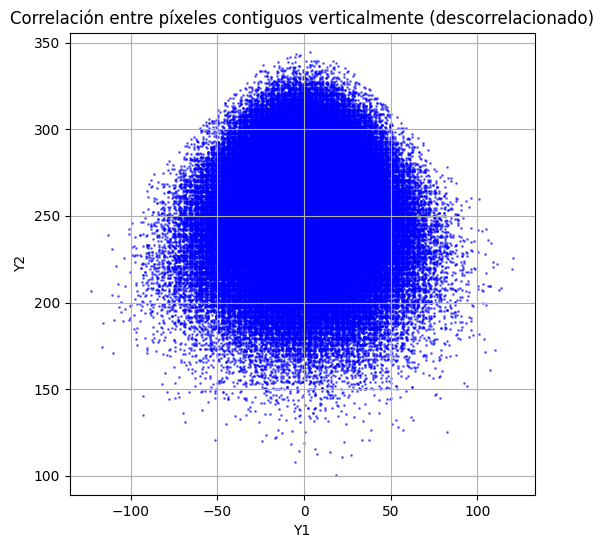
\includegraphics[width=0.7\textwidth]{Ejercicio1d.png}
    \caption{Imagen 2, gráfico de dispersión de la descorrelación de píxeles contiguos verticalmente}
    \label{fig:descorrelacion2}
\end{figure}

Por otro lado, en la segunda imagen, el gráfico se mantiene en forma de una nube, como en la Figura 2. Demostrando la falta de correlación inicial.

\section {Ejercicio 2: Compresión}

En este ejercicio se implementa un esquema de \textbf{compresión de imágenes} basado en el \textbf{Análisis de Componentes Principales (PCA)}. El objetivo de PCA es transformar un conjunto de datos

\[
X = \{\mathbf{x}_1, \mathbf{x}_2, \dots, \mathbf{x}_m\}, \quad \mathbf{x}_i \in \mathbb{R}^n,
\]

en un nuevo conjunto de variables

\[
Y = \{\mathbf{y}_1, \mathbf{y}_2, \dots, \mathbf{y}_m\}, \quad \mathbf{y}_i \in \mathbb{R}^k,
\]

mediante una transformación lineal tal que \(k < n\). Así, se logra \textbf{reducir la dimensionalidad} (de \(n\) a \(k\)), \textbf{descorrelacionar} las variables y conservar la mayor parte de la información relevante.

\subsubsection*{Formación de la matriz de datos}

La imagen se divide en sub-bloques de tamaño \(8 \times 8\) píxeles. Cada bloque se recorre por columnas y se aplana en un vector columna:

\[
\mathbf{x}_i = \mathrm{vec}(B^{(i)}) =
\begin{bmatrix}
B^{(i)}_{1,1} \\
B^{(i)}_{2,1} \\
\vdots \\
B^{(i)}_{8,1} \\
B^{(i)}_{1,2} \\
\vdots \\
B^{(i)}_{8,8}
\end{bmatrix}
\in \mathbb{R}^{64 \times 1}
\]

Repitiendo este proceso para todos los bloques, se obtiene una colección de vectores \(\mathbf{x}_1, \ldots, \mathbf{x}_m\), que se organizan como filas en la matriz de datos:

\[
X =
\begin{bmatrix}
\mathbf{x}_1^T \\
\mathbf{x}_2^T \\
\vdots \\
\mathbf{x}_m^T
\end{bmatrix}
\in \mathbb{R}^{m \times 64}
\]

Cada fila de \(X\) representa un bloque vectorizado de la imagen y cada columna una posición fija dentro del bloque.

\subsection*{Cálculo de la media y la matriz de covarianza}

La función \texttt{mean\_estimator()} calcula el vector media de las columnas de \(X\):

\[
\boldsymbol{\mu} = \frac{1}{m} \sum_{i=1}^m \mathbf{x}_i \in \mathbb{R}^{64}
\]

Luego, se centra la matriz de datos restando la media a cada fila:

\[
X_c = X - \mathbf{1}_m \boldsymbol{\mu}^T
\]

donde \(\mathbf{1}_m\) es un vector columna de unos de dimensión \(m\).

La función \texttt{cov\_estimator()} estima la matriz de covarianza:

\[
C_X = \frac{1}{m-1} X_c^T X_c \in \mathbb{R}^{64 \times 64}
\]

Cada elemento \(c_{ij}\) de \(C_X\) representa la covarianza entre la posición \(i\) y \(j\) dentro de los bloques.

\subsection*{Descomposición en autovalores y autovectores}

La función \texttt{pca\_transform()} aplica PCA resolviendo el siguiente problema de autovalores:

\[
C_X \mathbf{v}_j = \lambda_j \mathbf{v}_j, \quad j = 1, \dots, 64
\]

Se ordenan los autovalores \(\lambda_j\) en forma decreciente y se seleccionan los \(k\) mayores. Se construye la matriz de proyección:

\[
P = \begin{bmatrix} \mathbf{v}_1 & \mathbf{v}_2 & \cdots & \mathbf{v}_k \end{bmatrix} \in \mathbb{R}^{64 \times k}
\]

La representación reducida se obtiene como:

\[
Y = X_c P \in \mathbb{R}^{m \times k}
\]

El número de componentes \(k\) se define según el \textbf{factor de compresión}. En el código, la función \texttt{space\_saving\_k(s, m)} lo calcula como:

\[
k = \max\big(1, \min(m, \lceil m(1-s) \rceil)\big)
\]

donde \(s \in [0,1]\) es el porcentaje de reducción elegido.

\subsection*{Almacenamiento y reconstrucción}

La función \texttt{save\_data()} guarda:
\begin{itemize}
    \item \(Y\): matriz de datos comprimidos,
    \item \(P\): matriz de autovectores,
    \item \(\boldsymbol{\mu}\): vector de medias.
\end{itemize}

Esto permite reconstruir la aproximación de la imagen original con la fórmula inversa:

\[
\hat{X} = Y P^T + \mathbf{1}_m \boldsymbol{\mu}^T
\]

Finalmente, la función \texttt{plot\_eigenvalues()} grafica los autovalores \(\lambda_j\), destacando los conservados y los descartados.


\section {Ejercicio 3: Descompresión}

Luego de lo realizado en el Ejercicio 2, se realiza la reconstrucción de la imagen comprimida. Utilizando el proceso inverso del PCA de compresión, para descomprimir.
A través del Ejercicio 2, se obtienen los siguientes datos de la imagen:

Vectores \(y_i\) (\(Y\)), la matriz de autovectores (\(P\)) y la media \(\mu_X\) (\(\mu\))

Una vez obtenida la información indicada, se aplica la proyección inversa del PCA, para obtener los vectores \(x_i\) aproximados:

\[
X = Y P^T + \mu
\]
donde \(X\) es la matriz original, \(Y\) es la matriz proyectada, \(P\) son los autovectores y \(\mu\) es la media.
\\
Finalmente, se recorre una matriz vacía, del tamaño necesario de la imagen. Completando con los bloques de la imagen reconstruída.
De esta manera, obtenemos los siguientes resultados:

\begin{figure}[H]
    \centering
    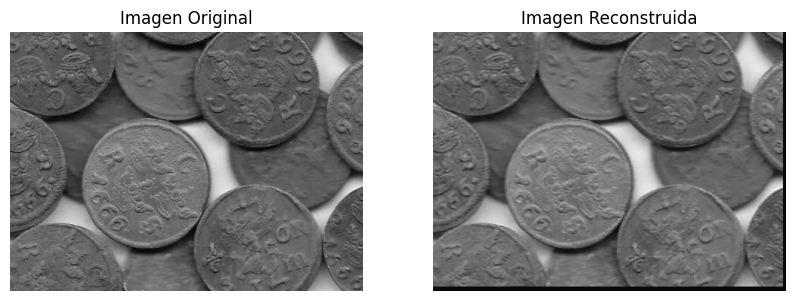
\includegraphics[width=1\textwidth]{Ejercicio3.png}
    \caption{Imagen reconstruida a través del proceso de PCA inverso.}
    \label{fig:ej3}
\end{figure}

Podemos notar el borde negro de la imagen reconstruida, lo cuál sucede al no poder completar bloques de exactamente 8 * 8 al comprimir la imagen.
Adicionalmente, podemos observar una diferencia entre las imágenes o pérdida de nitidez, atribuido a la reducción de la dimesionalidad y la eliminación de componentes de menor varianza.

\section{Ejercicio 4: Medidas de desempeño}
El objetivo de este ejercicio es evaluar el desempeño de la compresion de imagenes al variar el espacio ahorrado (S). 

\begin{equation}
S = \left( 1 - \frac{\text{cantidad de componentes principales } (k)}{\text{cantidad de componentes totales } (m)} \right) \times 100 \%
\end{equation}

En primer lugar, para cada porcentaje de espacio ahorrado comprimimos una imagen y la reconstruimos. Luego, para 
medir el rendimiento del procedimiento, calculamos el error cuadratico medio (MSE) entre la imagen original y 
la reconstruida. 
\begin{equation}
MSE = \frac{1}{N_w N_h} \sum_{i=1}^{N_w} \sum_{j=1}^{N_h} (p_{ij} - \hat{p}_{ij})^2
\end{equation}

\begin{figure}[H]
    \centering
    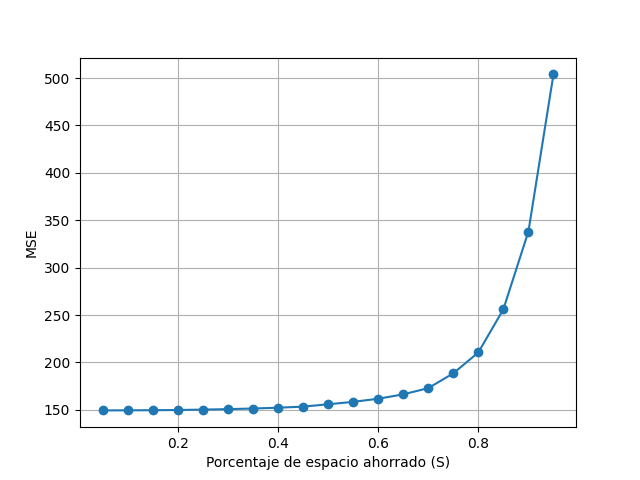
\includegraphics[width=1\textwidth]{Ejercicio 4a.png}
    \caption{Grafico MSE vs S}
    \label{fig:ej4}
\end{figure}

En el grafico, se observa que el error cuadratico medio aumenta a medida que lo hace el espacio ahorrado.
Este resultado es coherente, ya que al descartar un mayor numero de componentes principales se pierde mas 
informacion de la imagen. 
Sin embargo, esta relacion no es proporcional: el error crece considerablemente a partir de un espacio 
ahorrado del 80\%. Al superar ese porcentaje, la perdida de informacion se vuelve significativa, 
impactando notablemente en la calidad de la imagen. 


Para ilustrarlo, incluimos algunas imagenes para diferentes porcentajes de espacio ahorrado. 
\begin{figure}[H]
    \centering
    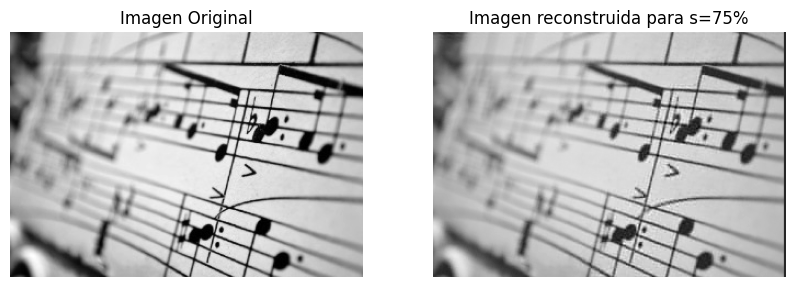
\includegraphics[width=1\textwidth]{Ejercicio 4b75.png}
    \caption{Imagenes original y reconstruida para un espacio ahorrado de 0.75.}
    \label{fig:ej4b1}
\end{figure}
\begin{figure}[H]
    \centering
    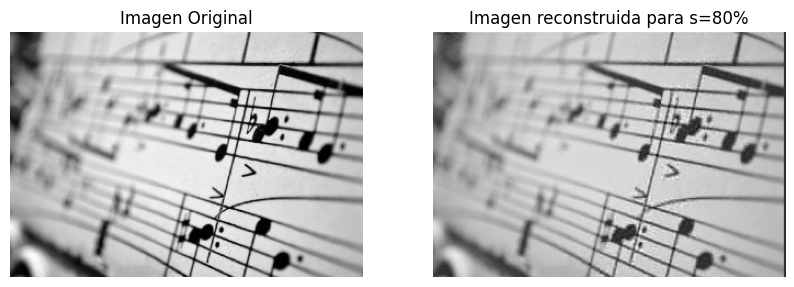
\includegraphics[width=1\textwidth]{Ejercicio 4b80.png}
    \caption{Imagenes original y reconstruida para un espacio ahorrado de 0.80.}
    \label{fig:ej4b2}
\end{figure}
\begin{figure}[H]
    \centering
    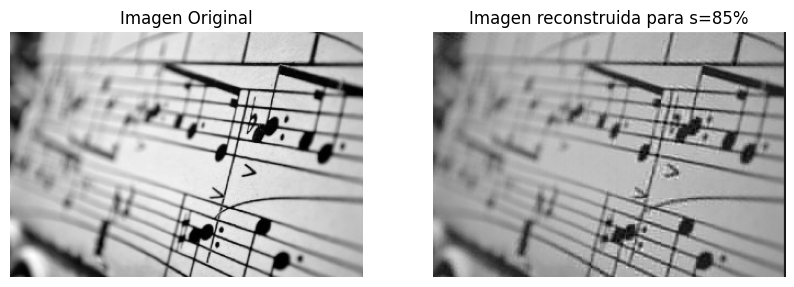
\includegraphics[width=1\textwidth]{Ejercicio 4b85.png}
    \caption{Imagenes original y reconstruida para un espacio ahorrado de 0.85.}
    \label{fig:ej4b3}
\end{figure}
\begin{figure}[H]
    \centering
    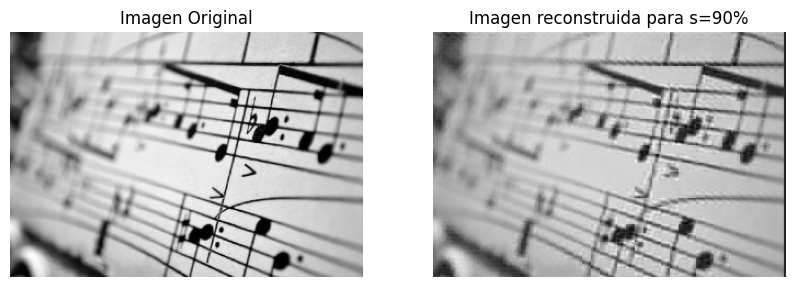
\includegraphics[width=1\textwidth]{Ejercicio 4b90.png}
    \caption{Imagenes original y reconstruida para un espacio ahorrado de 0.90.}
    \label{fig:ej4b4}
\end{figure}
\begin{figure}[H]
    \centering
    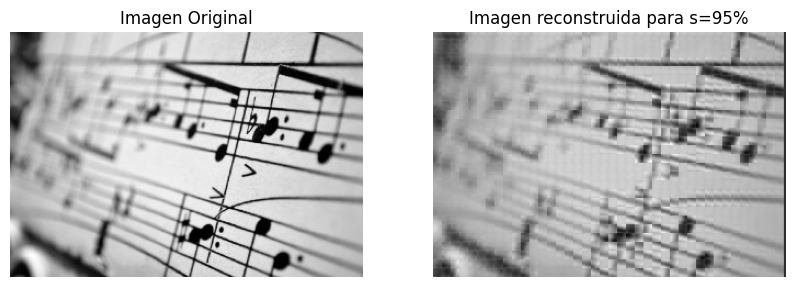
\includegraphics[width=1\textwidth]{Ejercicio 4b95.png}
    \caption{Imagenes original y reconstruida para un espacio ahorrado de 0.95.}
    \label{fig:ej4b5}
\end{figure}
Vemos que a medida que S aumenta, la imagen reconstruida pierde nitidez. La reduccion de 
componentes principales se ve en una disminucion de la calidad de la imagen. 

\section{Conclusiones}
En este trabajo practico implementamos y evaluamos la compresion de imagenes usando 
PCA (Analisis de Componentes Principales). Este permite reducir la dimension de los datos
al descartar las componentes de menor varianza, quedandose con las componentes principales, 
es decir aquellas necesarias para la comprension de la imagen. De esta manera, se ahorra espacio 
sin compromenter significativamente la calidad de la imagen .

Los resultados mostraron que, a medida que aumenta el porcentaje de espacio ahorrado, la calidad
de la imagen reconstruida decae progresivamente, especialmente a partir de la reducicon de 80\%. 
Esto se refleja en un incremento notable del MSE. Sin embargo, consideramos que
para valores intermedios de compresion (cercanos al 70\%), obtenemos un buen balance entre nitidez 
de la imagen y reduccion de memoria. 

* parrafo de dificultades *

En conclusion, la aplicacion de PCA para la compresion de imagenes nos permitio observar
de primera mano como la reduccion de dimensionalidad ayuda en el ahorro de almacenamiento,
sin comprometer demasiado la calidad de la imagen.




\section*{Referencias}
\addcontentsline{toc}{section}{Referencias}
\bibliographystyle{plain}
\bibliography{referencias}

\end{document}